%!TEX encoding = UTF-8 Unicode
%!TEX root = ../livre-can.tex

%-----------------------------------------------------------

\newcommand\controleurCAN {
  \draw (1, 0) node [above] {\small\tt TxD} ;
  \draw (2, 0) node [above] {\small\tt RxD} ;
  \draw[very thick] (0, 1.5) -- ++ (0, -1.5) -- ++ (3, 0) -- ++ (0, 1.5) ;
}

\newcommand\PMPorteEt[1] {
  \draw[very thick, line cap=round, fill=white]
     (0, #1) 
     -- ++(#1, 0)
     arc (90:-90:#1)
     -- ++(-#1, 0)
     -- cycle ;
}

\newcommand\PMPoint[2] {
  \draw (#1, #2)[fill=black] circle (.05) ;
}

\newcommand\PMResistance[3] {
  \draw (#1, #2 - .5) -- ++ (0, 1) ;
  \draw (#1 - .1, #2 - .25) [fill=white] rectangle (#1 + .1, #2 + .25) ;
  \draw (#1, #2) node {\small\tt #3} ;
}

%-----------------------------------------------------------

\chapter{Architecture}

%--- Pour supprimer tout en-tête et pied de page sur la 1re page d'un chapitre
\thispagestyle{empty}



\begin{figure}[ht]
  \centering
  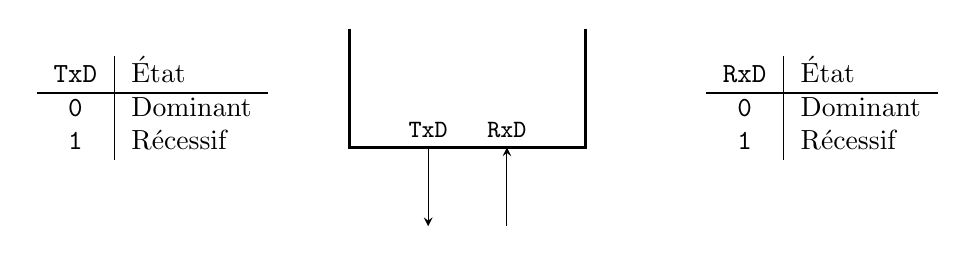
\begin{tikzpicture}[>=stealth]
   \controleurCAN
   \draw (2, -1)[->] -- ++ (0, 1) ;
   \draw (1, 0) [->] -- ++ (0, -1) ;
    \draw (-2.5, .5) node {
      \begin{tabular}{c|l}
        \texttt{TxD} & État \\
        \hline
        \texttt{0} & Dominant \\
        \texttt{1} & Récessif \\
      \end{tabular}
    } ;
    \draw (6, .5) node {
      \begin{tabular}{c|l}
        \texttt{RxD} & État \\
        \hline
        \texttt{0} & Dominant \\
        \texttt{1} & Récessif \\
      \end{tabular}
    } ;
  \end{tikzpicture}
  \caption{Contrôleur CAN}
  \labelFigure{figureControleurSortieDeuxEtats}
\end{figure}


\begin{figure}[ht]
  \centering
  \begin{tikzpicture}[>=stealth]
   \controleurCAN
   \draw (2, -1)[->] -- ++ (0, 1) ;
   \draw (1, 0) [triangle 90 reversed->] -- ++ (0, -1) ;
    \draw (-2.5, .5) node {
      \begin{tabular}{c|l}
        \texttt{TxD} & État \\
        \hline
        \texttt{0} & Dominant \\
        \texttt{Hi-Z} & Récessif \\
      \end{tabular}
    } ;
    \draw (6, .5) node {
      \begin{tabular}{c|l}
        \texttt{RxD} & État \\
        \hline
        \texttt{0} & Dominant \\
        \texttt{1} & Récessif \\
      \end{tabular}
    } ;
  \end{tikzpicture}
  \caption{Contrôleur CAN}
  \labelFigure{figureControleurSortieTroisEtats}
\end{figure}




\begin{figure}[ht]
  \centering
  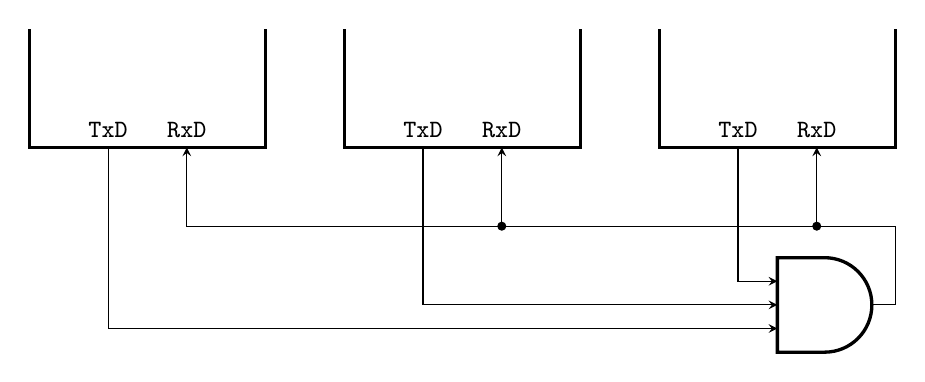
\begin{tikzpicture}[>=stealth]
    \controleurCAN
   \begin{scope}[xshift=4cm]
     \controleurCAN
   \end{scope}
   \begin{scope}[xshift=8cm]
     \controleurCAN
   \end{scope}
   \draw (9, 0)[->] -- ++ (0, -1.7) -- ++ (.5, 0);
   \draw (5, 0)[->] -- ++ (0, -2) -- ++ (4.5, 0);
   \draw (1, 0)[->] -- ++ (0, -2.3) -- ++ (8.5, 0);
   \draw (10.5, -2)[->] -- ++ (.5, 0) -- ++ (0, 1) -- ++ (-9, 0) -- ++ (0, 1) ;
   \draw (6, -1)[->] -- ++ (0, 1) ;
   \PMPoint{6}{-1}
   \PMPoint{10}{-1}
   \draw (10, -1)[->] -- ++ (0, 1) ;
   \begin{scope}[xshift=9.5cm, yshift=-2cm]
     \PMPorteEt{.6}
   \end{scope}
  \end{tikzpicture}
  \caption{Simple réseau}
  \labelFigure{figureReseauPorteEt}
\end{figure}



\begin{figure}[ht]
  \centering
  \begin{tikzpicture}[>=stealth]
    \controleurCAN
   \begin{scope}[xshift=4cm]
     \controleurCAN
   \end{scope}
   \begin{scope}[xshift=8cm]
     \controleurCAN
   \end{scope}
   \draw (.5, -1) -- ++ (10, 0) ;
   \draw (1, 0)[triangle 90 reversed ->] -- ++ (0, -.95) ;
   \draw (2, -1)[->] -- ++ (0, 1) ;
   \PMPoint{1}{-1}
   \PMPoint{2}{-1}
   \draw (5, 0)[triangle 90 reversed->] -- ++ (0, -.95) ;
   \draw (6, -1)[->] -- ++ (0, 1) ;
   \PMPoint{5}{-1}
   \PMPoint{6}{-1}
   \draw (9, 0)[triangle 90 reversed->] -- ++ (0, -.95) ;
   \draw (10, -1)[->] -- ++ (0, 1) ;
   \PMPoint{9}{-1}
   \PMPoint{10}{-1}
   \PMResistance{.5}{-1.5}{R}
   \PMResistance{10.5}{-1.5}{R}
   \draw (.5, -2) node [below] {\tiny\tt $V_{CC}$} ;
   \draw (10.5, -2) node [below] {\tiny\tt $V_{CC}$} ;
  \end{tikzpicture}
  \caption{Simple réseau}
  \labelFigure{figureReseauOpenCollector}
\end{figure}


\section{Transcepteur CAN}



